\let\negmedspace\undefined
\let\negthickspace\undefined
\documentclass[journal]{IEEEtran}
\usepackage[a5paper, margin=10mm, onecolumn]{geometry}
%\usepackage{lmodern} % Ensure lmodern is loaded for pdflatex
\usepackage{tfrupee} % Include tfrupee package

\setlength{\headheight}{1cm} % Set the height of the header box
\setlength{\headsep}{0mm}     % Set the distance between the header box and the top of the text

\usepackage{gvv-book}
\usepackage{gvv}
\usepackage{cite}
\usepackage{amsmath,amssymb,amsfonts,amsthm}
\usepackage{algorithmic}
\usepackage{graphicx}
\usepackage{textcomp}
\usepackage{xcolor}
\usepackage{txfonts}
\usepackage{listings}
\usepackage{enumitem}
\usepackage{mathtools}
\usepackage{gensymb}
\usepackage{comment}
\usepackage[breaklinks=true]{hyperref}
\usepackage{tkz-euclide} 
\usepackage{listings}
% \usepackage{gvv}                                        
\def\inputGnumericTable{}                                 
\usepackage[latin1]{inputenc}                                
\usepackage{color}                                            
\usepackage{array}                                            
\usepackage{longtable}                                       
\usepackage{calc}                                             
\usepackage{multirow}                                         
\usepackage{hhline}                                           
\usepackage{ifthen}                                           
\usepackage{lscape}
\begin{document}
\bibliographystyle{IEEEtran}
\vspace{3cm}

\title{CHAPTER - 1\\Vector Arithmetic}
\author{EE24BTECH11061 - Rohith Sai}
\maketitle

\renewcommand{\thefigure}{\theenumi}
\renewcommand{\thetable}{\theenumi}

\section{1.8 Length}
\begin{enumerate}
\item [1.8.9] Find the values of $y$ for which the distance between the points $\vec{P}(2, -3)$ and $\vec{Q}(10, y)$ is $10$ units.\\
\textbf{Solution:}
Given points $\vec{P}$ and $\vec{Q}$ are represented as:
\begin{align}
    \vec{P} = \myvec{
2 \\ -3
}
\end{align}
\begin{align}
    \vec{Q} = \myvec{
    10 \\ y
    }
\end{align}
Let the distance between the two points be $d$.
Given that the distance between the two points $\vec{P}$ and $\vec{Q}$ is $10$ units:
\begin{align}
    d=10
\end{align}
We know that $d$ is defined as:
\begin{align}
    d = \abs{\abs{\vec{P}-\vec{Q}}}\\
    \implies d = \sqrt{{\brak{\vec{P}-\vec{Q}}}^\top\brak{\vec{P}-\vec{Q}}}
\end{align}
\begin{align}
    \vec{P} - \vec{Q} = \myvec{2\\-3} - \myvec{10\\y} = \myvec{-8\\-3-y}\\
\end{align}
From $(3)$:
\begin{align}
    d = \abs{\abs{\vec{P}-\vec{Q}}} = 10\\
    \implies {\brak{\vec{P}-\vec{Q}}}^\top\brak{\vec{P}-\vec{Q}} = 100
\end{align}
Therefore:
\begin{align}
    y = 3 \text{ and } y = -9
\end{align}
\begin{figure}[htp]
    \centering
    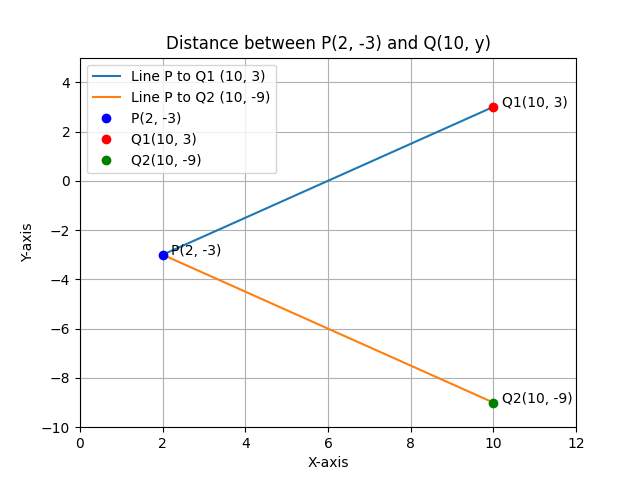
\includegraphics[width=10cm]{figs/figure.png}
    \label{fig:figure}
\end{figure}
\end{enumerate}
\end{document}